\documentclass[10pt,a4paper, twocolumn, conference]{IEEEtran}
\author{Adam Lee}
\title{Simple Linear Regression - A Journey Begins}
\date{November 2020}
\usepackage{pgfplots}
\usepackage{graphicx}
\usepackage{float}
\usepackage{amsmath}
\usepackage{amsfonts}
\usepackage{amssymb}
\usepackage{verbatim}
\usepackage{amsbsy}
\usepackage{algorithm}
\usepackage{algorithmic}
\usepackage[T1]{fontenc}
\usepackage[utf8]{inputenc}
\usepackage{hyperref}
\usepackage{cleveref}
\usepackage{placeins}
\usepackage{subcaption}
\usepackage{tablefootnote}
\DeclareMathOperator{\var}{var}
\renewcommand{\tabcolsep}{18pt}
\begin{document}
\maketitle
\pagebreak
\section{Introduction}
Regression is a statistical tool used in many facets of data analysis.  Wherever correlated data is concerned, regression methods are often used to effectively and efficiently describe trends between two or more variables. During my brief first insights into machine learning, the initial bridge between statistics and machine learning has been linear regression. In its most simple form, a linear regression model assumes the relationship between a set of dependent variables $\mathbf{y} = \left[ y_1, \ldots, y_n \right] ^{\text{T}}$ and a set of independent variables $\mathbf{x} = \left[ \mathbf{x}_1, \ldots, \mathbf{x}_n \right] ^{\text{T}}$ is linear. Here each independent variable $\mathbf{x}_i \in \mathbb{R}^{D}$ is a $D$ dimension vector of real valued inputs, however for our simple model we consider the case where $x_i \in \mathbb{R}$ such that the \textbf{simple linear regression model} has the form
\begin{equation} \label{eq1}
\mathbf{y} = \beta_0 + \beta_1 \mathbf{x} + \boldsymbol\varepsilon,
\end{equation}
where $\mathbf{y}$ is our vector of response variables and $\mathbf{x}$ is the vector of single regressors. The intercept of this model $\beta_0$ and the slope $\beta_1$ are unknown constants and associated error term $\boldsymbol\varepsilon$ is treated as a random variable.
\vspace{3mm}
\hrule
\begin{figure}[h]
\begin{center}
\begin{minipage}{0.24\textwidth}
\begin{center}
\includegraphics[width=1.0\textwidth]{data_graph0}
\end{center}
\label{fig:first}
\end{minipage}
\begin{minipage}{0.24\textwidth}
\begin{center}
\includegraphics[width=1.0\textwidth]{data_graph1}
\end{center}
\label{fig:second}
\end{minipage}
\caption{A scatter-plot of data (left) and an example of a linear regression model (right)}
\label{fig:1}
\end{center}
\end{figure}
\hrule
\vspace{3mm}
We can consider the error term $\varepsilon$ to be a statistical error. Therefore, it accounts for the failure of the model to fit the data exactly. It is common to assume the error term $\varepsilon$ is Gaussian with mean $\mu = 0$ and variance $\var(\varepsilon) = \sigma^2$. Assume further that our regressor variable $x$ is fixed, such that the response variable $y$ is now dependant only on $\varepsilon$. Then our mean response variable at any value of $x$ is given by
\begin{equation}
\mathcal{E}[y|x] = \mu_{y|x} = \beta_0 + \beta_1 x
\end{equation}
with variance
\begin{equation}
\var(y|x) = \sigma_{y|x}^2 = \sigma^2.
\end{equation}
Therefore, we can consider the true regression model $\mu_{y|x}$ to be a function of mean values such that
\begin{equation}
\mu_{y|x}(x_{n+1}) = \beta_0 + \beta_1 x_{n+1} = y_{n+1},
\end{equation}
is the expected value $y_{n+1}$ for a new prediction variable $x_{n+1}$ to the data set $\mathbf{x}$. The variance of $y_i$ at a given $x_i$ is thus determined by $\sigma^2$. We see this model in~\cref{fig:figure2}, with two example training points and our prediction point $x_{n+1}$.

In general, the response variable $y$ may be related to multiple regressors. Say we have a relation between $d$ regressors then
\begin{equation}
y = \beta_0 + \sum_{i = 1}^d \beta_i x_i + \varepsilon.
\end{equation}
This is known as multiple-linear regression and will be discussed in full later.

Clearly, the aim of both simple and multiple linear regression is to minimise the error term $\varepsilon$ such that we have a model which best fits our observed data.
\vspace{2mm}
\hrule
\begin{figure}[H]
\centering
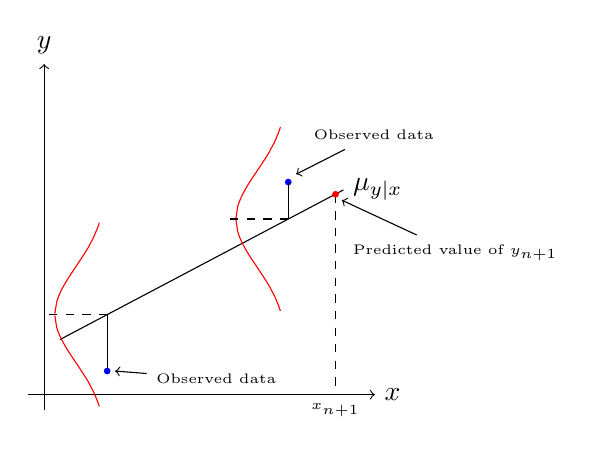
\begin{tikzpicture}[domain = 0:4]
\draw[->] (-0.2,0) -- (4.2,0) node[right] {$x$};
\draw[->] (0,-0.2) -- (0,4.2) node[above] {$y$};
\draw[-] (0.2, 0.7) -- (3.8,2.6) node[right] {$\mu_{y|x}$};
\draw[-] (0.8,0.3) -- (0.8, 1.01667);
\draw[dashed] (0.8,1.01667) -- (-0.0, 1.01667);
\draw[dashed] (3.7, 2.54) -- (3.7, 0.0);
\node[anchor = south] (x0) at (3.7,-0.4) {\tiny{$x_{n+1}$}};
\filldraw[color = blue]
(0.8,0.3) circle (1pt);
\draw[domain = 0.135:0.7, color = red] plot (\x, {1.01667 - 0.6*sqrt( -ln(2*3.14*0.6*0.6*(\x - 0.8)^2 ) )});
(0.8,0.3) circle (1pt);
\draw[domain = 0.135:0.7, color = red] plot (\x, {1.01667 + 0.6*sqrt( -ln(2*3.14*0.6*0.6*(\x - 0.8)^2 ) )});
\filldraw[color = blue]
(3.1, 2.7) circle (1pt);
\filldraw[color = red]
(3.7, 2.545) circle (1pt);
\draw[-] (3.1, 2.7 - 0.4695) -- (3.1, 2.7); 
\draw[dashed] (3.1, 2.2305) -- (2.3, 2.2305);
\draw[domain = 2.435:2.435+0.565, color = red] plot (\x, {2.2305 - 0.6*sqrt( -ln(2*3.14*0.6*0.6*(\x - 3.1)^2 ) )});
\draw[domain = 2.435:2.435+0.565, color = red] plot (\x, {2.2305 + 0.6*sqrt( -ln(2*3.14*0.6*0.6*(\x - 3.1)^2 ) )});
\node[anchor  = west] (x1) at (1.3, 0.2) {\tiny{Observed data}};
\draw[->] (x1) to (0.9, 0.3);
\node[anchor = west] (x2) at (3.3, 3.3) {\tiny{Observed data}};
\draw[->] (x2) to (3.2, 2.8);
\node[anchor = west] (x3) at (3.8, 1.8) {\tiny{Predicted value of $y_{n+1}$}};
\draw[->] (x3) to (3.78, 2.47);
\end{tikzpicture}
\caption{A visual representation of simple linear regression}
\label{fig:figure2}
\end{figure}
\hrule
\vspace{2mm}
\section{Simple Linear Regression}
Let us first consider the case of simple linear regression, such that we have a single response variable $y$ and a single regressor $x_1 := x$. Our initial model, as we have discussed, is
\begin{equation}
y = \beta_0 + \beta_1 x + \epsilon,
\end{equation}
where the intercept $\beta_0$ and the slope $\beta_1$ are unknown constants and the error term $\varepsilon$ is a random variable. The parameters $\beta_{0,1}$ must be determined by sampling data and we will consider methods for doing so in later sections. These parameters are known as the regression coefficients and have a very simple practical interpretation. The slope $\beta_1$ is the expected change in value of $y$ per unit change in value of $x$. The intercept $\beta_0$ is the expected value of the response given the value of the regressor is zero.
\subsection{Least Squares method for parameter estimation}
As we mentioned, the parameters $\beta_{0,1}$ are unknown constants and must be estimated using the sample data we have collected. The \textit{method of least squares} allows us to do so. Let us adopt the notation that our data set $\varkappa$ is a collection of sample pairs
\begin{equation}
\varkappa = \{ (x_0, y_0), \ldots, (x_k, y_k) \}.
\end{equation}
We can input this data into \cref{eq1} to obtain a system of equations
\begin{equation}
y_i = \beta_0 + \beta_1 x_i + \varepsilon_i,~~i = 0, \ldots, k.
\end{equation}
Let us define the Least Squares criterion function
\begin{equation}
\mathbf{E}(\beta_0, \beta_1) := \sum_{i=0}^k (y_i - \beta_0 - \beta_1 x_i)^2.
\end{equation}
Let us further introduce real constants $\hat{\beta_0}, \hat{\beta_1}$ which satisfy the minima conditions
\begin{align} \label{al1} \nonumber
\frac{\partial \mathbf{E}}{\partial \beta_0} \Big|_{\hat{\beta_0}, \hat{\beta_1}} & = -2 \sum_{i=0}^k (y_i - \hat{\beta_0} - \hat{\beta_1}x_i) = 0 \\
\frac{\partial \mathbf{E}}{\partial \beta_1} \Big|_{\hat{\beta_0}, \hat{\beta_1}} & = -2 \sum_{i=0}^k (y_i - \hat{\beta_0} - \hat{\beta_1}x_i)x_i = 0
\end{align}
We can simplify \cref{al1} to gain the least squares normal equations
\begin{align}
\nonumber
(k + 1) \hat{\beta_0} + \hat{\beta_1} \sum_{i=0}^k x_i & = \sum_{i=0}^k y_i, \\
 \hat{\beta_0} \sum_{i=0}^k x_i + \hat{\beta_1} \sum_{i=0}^k (x_i)^2 & = \sum_{i=0}^k y_i x_i.
\end{align}
We can solve the first of the pair of equations for $\hat{\beta_0}$
\begin{equation} \label{eq12}
\hat{\beta_0} =\bar{y} - \hat{\beta_1} \bar{x},
\end{equation}
where $\bar{a} := \frac{1}{k+1} \sum_{i = 0}^k a_i$ is the average value of all data points $a_i$. We now solve the second equation by substituting in \cref{eq12} as follows
\begin{equation} \label{eq13}
(\bar{y} - \hat{\beta_1} \bar{x}) \sum_{i=0}^k x_i + \hat{\beta_1} \sum_{i=0}^k x_i^2 = \sum_{i=0}^k x_i y_i,
\end{equation}
and then solving with respect to $\hat{\beta_1}$ we obtain
\begin{equation}
\hat{\beta_1} = \frac{\sum_{i=0}^k x_i y_i - \frac{\sum_{i = 0}^k x_i y_i}{k + 1}}{\sum_{i=0}^k x_i^2 - \frac{\sum_{i=0}^k x_i^2}{k+1}}.
\end{equation}
The numerator of \cref{eq13} is nothing other than the corrected sum of dot products between $x_i$ and $y_i$, while the denominator is the corrected sum of squares for $x_i$ and thus we can introduce a concise notation for $\hat{\beta_1}$, namely
\begin{equation}
\hat{\beta_1} = \frac{\sum_{i=0}^k y_i (x_i - \bar{x})}{\sum_{i=0}^k (x_i - \bar{x})^2} = \frac{S_{xy}}{S_{xx}}.
\end{equation}
Then, our fitted simple linear regression model is nothing else than
\begin{equation}
\hat{y} = \hat{\beta_0} + \hat{\beta_1} x.
\end{equation}
\section{Example 1}
Constructing an example for the method of least squares is quite simple. Consider the data-set \cref{fig:dat}, where each $y_i$ was sampled from a normal distribution centred on $x_i$ with uniform variance $\sigma^2 = 2$
\vspace{2mm}
\hrule
\begin{figure}[H]
\centering
\begin{tabular}{c|c|c}
Observation, $i$ & $x_i$ & $y_i$ \\
\hline
\hline
1 &1&0.5678 \\
2 &2&1.3519 \\
3 &3&3.1623 \\
4 &4&6.7229 \\
5 &5&5.0327 \\
6 &6&5.9015 \\
7 &7&7.1302 \\
8 &8&6.7212 \\
9 &9&9.6973 \\
10 &10&9.3017 \\
11 &11&10.7025 \\
12 &12&12.0149 \\
13 &13&12.3884 \\
14 &14& 16.5306\\
15 &15&15.9602 \\
\end{tabular}
\caption{\small{Example data set}}
\label{fig:dat}
\end{figure}
\hrule
\vspace{2mm}
The general trend for this data is clear, and from the distribution we used to generate the samples $y_i$ we would expect the parameter values to be $\hat{\beta_0} \approx 0$ and $\hat{\beta_1} \approx 1$. Quick calculation concludes that we have
\begin{equation}
\hat{\beta_1} = \frac{S_{xy}}{S_{xx}} = \frac{292.5196}{280.00} \approx 1.0447.
\end{equation}
Then we have
\begin{align} \nonumber
\hat{\beta_0} & = \bar{y} - \beta_1 \bar{x} \\
 & = 8.2118 - 1.0447 \cdot 8  \approx -0.1459.
\end{align}
We have our two parameters $\hat{\beta_0}, \hat{\beta_1}$ and can fit our regression line $\hat{y}$ accordingly. We refer back to our expectations for these values, and conclude this would be an appropriate regression line for this simple case. This example is in fact the same as \cref{fig:1}, we present the figure again in \cref{fig:main}, extending the regression line to observe the $y$-intercept clearly.
\pagebreak
\onecolumn
\begin{figure}[H]
\centering
\includegraphics[width = 1.0\textwidth]{data_graphmain}
\caption{The scatterplot for \cref{fig:dat} with regression line $\hat{y}$ in red.}
\label{fig:main}
\end{figure}




\end{document}